% ============================================================================
% CHAPTER 2: SUPERVISED LEARNING AND CURVE FITTING
% ============================================================================

\chapter{Supervised Learning and Curve Fitting}
\label{ch:supervised_learning}

% ============================================================================
% OVERVIEW
% ============================================================================

\section{Chapter Overview}

This chapter introduces supervised learning through the lens of \textbf{curve fitting}---one of the simplest yet most illustrative examples in machine learning. We will explore how data is generated, what patterns and noise mean, how to fit mathematical functions to data, and the fundamental tension between fitting data well (minimizing error) and generalizing to new, unseen examples.

\textbf{Learning Objectives:}
\begin{itemize}
    \item Understand how real-world data combines patterns and noise
    \item Formulate curve fitting as an optimization problem
    \item Define and compute error functions (squared error, MSE, RMSE)
    \item Distinguish between underfitting, good fit, and overfitting
    \item Introduce regularization as a solution to overfitting
    \item Understand the role of hyperparameters and validation
\end{itemize}

% ============================================================================
% DATA: PATTERNS AND NOISE
% ============================================================================

\section{Understanding Data: Patterns and Noise}

\subsection{Data as Information}

In machine learning, data is the raw material from which we extract knowledge. Each data point carries \textit{information}---the degree to which observing that data point changes what we know about the world.

\begin{bluebox}[Information as Surprise]
The concept of \textbf{information} is deeply connected to \textbf{surprise}:
\begin{itemize}
    \item If you observe something you already expected, you gain little information.
    \item If you observe something unexpected, you gain more information.
\end{itemize}

This intuition forms the basis of \textbf{information theory}, which we'll explore later. For now, understand that data contains hidden patterns that we wish to discover.
\end{bluebox}

\subsection{The Generating Process}

We assume that data comes from some underlying \textbf{generating process} or \textbf{distribution}. This distribution is typically \textit{unknown}---if we knew it, there would be no need for machine learning!

\begin{center}
\begin{tikzpicture}[
    box/.style={draw, rounded corners, minimum width=3cm, minimum height=1.2cm, align=center, fill=blue!10},
    arrow/.style={-Stealth, thick}
]
    \node[box, fill=purple!20] (dist) at (0,0) {Unknown\\Distribution $P$};
    \node[box, fill=green!20] (pattern) at (5,0.8) {Pattern\\(Signal)};
    \node[box, fill=red!20] (noise) at (5,-0.8) {Noise\\(Random)};
    \node[box, fill=orange!20] (data) at (10,0) {Observed\\Data};
    
    \draw[arrow] (dist) -- (pattern);
    \draw[arrow] (dist) -- (noise);
    \draw[arrow] (pattern) -- (data);
    \draw[arrow] (noise) -- (data);
\end{tikzpicture}
\end{center}

\subsection{Pattern vs. Noise}

Real-world data consists of two components:

\begin{enumerate}
    \item \textbf{Pattern (Signal)}: The underlying regularity or structure we want to learn. This is captured by some function $g(\vect{x})$.
    
    \item \textbf{Noise}: Random variations that obscure the pattern. Noise arises from:
    \begin{itemize}
        \item Measurement errors
        \item Intrinsic randomness in the process
        \item Unobserved variables affecting the outcome
    \end{itemize}
\end{enumerate}

\begin{definitionbox}[Data Generation Model]
In a typical supervised learning scenario, targets are generated as:
\[
t = g(\vect{x}) + \epsilon
\]
where:
\begin{itemize}
    \item $g(\vect{x})$ is the true (unknown) generating function
    \item $\epsilon$ is noise, often assumed to be $\epsilon \sim \mathcal{N}(0, \sigma^2)$ (Gaussian with mean 0)
\end{itemize}
\end{definitionbox}

\textbf{Our Goal}: Learn the pattern $g(\vect{x})$ while ignoring the noise.

% ============================================================================
% SYNTHETIC DATA EXAMPLE
% ============================================================================

\section{Synthetic Data Generation}

To understand supervised learning concretely, let's work with synthetic data where we know the true generating function.

\subsection{The Setup}

Consider:
\begin{itemize}
    \item Input variable: $x \in [0, 1]$
    \item Target variable: $t \in \R$
    \item Generating function: $g(x) = \sin(2\pi x)$
    \item Noise: $\epsilon \sim \mathcal{N}(0, 0.1^2)$
\end{itemize}

Thus, the observed targets are:
\[
t_n = \sin(2\pi x_n) + \epsilon_n
\]

\subsection{Python Code for Data Generation}

\begin{lstlisting}[language=Python, caption=Synthetic Data Generation]
import numpy as np
import matplotlib.pyplot as plt

def generate_synthetic_data(n, noise_std=0.1, random_seed=None):
    """Generate synthetic data from sin(2*pi*x) with Gaussian noise."""
    if random_seed is not None:
        np.random.seed(random_seed)
    
    # Generate uniformly spaced x values in [0, 1]
    x = np.linspace(0, 1, n)
    
    # Compute the true target (the pattern)
    t_true = np.sin(2 * np.pi * x)
    
    # Add Gaussian noise
    noise = np.random.normal(0, noise_std, n)
    t = t_true + noise
    
    return x, t
\end{lstlisting}

\begin{bluebox}[Why Synthetic Data?]
By using synthetic data where we know the true generating function:
\begin{enumerate}
    \item We can \textbf{verify} whether our learned model approximates the true function
    \item We can \textbf{visualize} the gap between predictions and truth
    \item We can \textbf{control} the noise level to study its effects
\end{enumerate}

In real applications, we never know $g(\vect{x})$---this is precisely what we're trying to learn!
\end{bluebox}

% ============================================================================
% THE SUPERVISED LEARNING PROBLEM
% ============================================================================

\section{The Supervised Learning Problem}

\subsection{Problem Formulation}

We have:
\begin{itemize}
    \item A \textbf{training set}: $\mathcal{D} = \{(x_1, t_1), (x_2, t_2), \ldots, (x_N, t_N)\}$
    \item Input features: $x_n$ (known)
    \item Targets: $t_n$ (known for training data)
\end{itemize}

\textbf{Goal}: Learn a function $y(x; \vect{w})$ that predicts targets for \textit{new, unseen} inputs.

\begin{center}
\begin{tikzpicture}[
    box/.style={draw, rounded corners, minimum width=2.5cm, minimum height=1cm, align=center, fill=gray!10},
    arrow/.style={-Stealth, thick}
]
    \node[box, fill=blue!20] (train) at (0,0) {Training Data\\$(x_n, t_n)$};
    \node[box, fill=green!20] (algo) at (4,0) {Learning\\Algorithm};
    \node[box, fill=orange!20] (model) at (8,0) {Learned Model\\$y(x; \vect{w}^*)$};
    \node[box, fill=red!20] (new) at (4,-2.5) {New Input\\$x_{\text{new}}$};
    \node[box, fill=purple!20] (pred) at (8,-2.5) {Prediction\\$\hat{t}_{\text{new}}$};
    
    \draw[arrow] (train) -- (algo);
    \draw[arrow] (algo) -- (model);
    \draw[arrow] (new) -- (pred);
    \draw[arrow] (model) -- (pred);
\end{tikzpicture}
\end{center}

\subsection{Generalization: The Key Challenge}

The core difficulty is that we have \textbf{finite data} but want to make predictions for \textbf{infinitely many possible inputs}. This requires \textbf{generalization}---the model must capture the underlying pattern, not memorize the training examples.

\begin{importantbox}[The Generalization Principle]
\textbf{We want to generalize, not memorize.}

A model that perfectly fits training data but fails on new data has \textit{memorized} rather than \textit{learned}. The true test of learning is performance on unseen data.
\end{importantbox}

% ============================================================================
% CURVE FITTING
% ============================================================================

\section{Curve Fitting: A Polynomial Approach}

\subsection{Polynomial Basis Functions}

One of the simplest approaches to fitting a function is using \textbf{polynomials}. We express our model as:

\begin{definitionbox}[Polynomial Model]
\[
y(x; \vect{w}) = w_0 + w_1 x + w_2 x^2 + \cdots + w_M x^M = \sum_{j=0}^{M} w_j x^j
\]
where:
\begin{itemize}
    \item $M$ is the \textbf{degree} of the polynomial
    \item $\vect{w} = (w_0, w_1, \ldots, w_M)^\top$ are the \textbf{coefficients} (parameters) to learn
\end{itemize}
\end{definitionbox}

\begin{bluebox}[Why Polynomials?]
\begin{itemize}
    \item \textbf{Universal Approximation}: By Taylor's theorem, any smooth function can be approximated arbitrarily well by a polynomial of sufficient degree.
    \item \textbf{Linear in Parameters}: Although $y(x; \vect{w})$ is nonlinear in $x$, it is \textit{linear in $\vect{w}$}. This makes optimization tractable.
    \item \textbf{Simple to Understand}: Polynomials provide intuitive examples for understanding key concepts.
\end{itemize}
\end{bluebox}

\subsection{Choosing the Polynomial Degree}

The degree $M$ controls model complexity:
\begin{itemize}
    \item $M = 0$: Constant (horizontal line)
    \item $M = 1$: Linear (straight line)
    \item $M = 2$: Quadratic (parabola)
    \item $M = 3$: Cubic
    \item Higher $M$: More complex curves
\end{itemize}

As $M$ increases, the polynomial gains more \textbf{degrees of freedom} to fit the data.

\subsection{The ``Curve Fitting Machine'' Analogy}

Imagine a machine with \textbf{knobs} labeled $w_0, w_1, \ldots, w_M$. By adjusting these knobs, we change the shape of the curve. Our goal is to find the knob settings that make the curve pass as close as possible to all data points.

\begin{center}
\begin{tikzpicture}[
    knob/.style={circle, draw, fill=blue!20, minimum size=0.8cm, font=\small}
]
    \node[draw, rounded corners, minimum width=6cm, minimum height=3cm, fill=gray!10] (machine) at (0,0) {};
    \node at (0,1) {\textbf{Curve Fitting Machine}};
    
    \node[knob] at (-2,-0.5) {$w_0$};
    \node[knob] at (-0.7,-0.5) {$w_1$};
    \node[knob] at (0.6,-0.5) {$w_2$};
    \node at (1.6,-0.5) {$\cdots$};
    \node[knob] at (2.3,-0.5) {$w_M$};
    
    \draw[-Stealth, thick] (-4,0) -- (-3.2,0) node[midway, above] {Data};
    \draw[-Stealth, thick] (3.2,0) -- (4,0) node[midway, above] {Curve};
\end{tikzpicture}
\end{center}

% ============================================================================
% ERROR FUNCTIONS
% ============================================================================

\section{Error Functions: Quantifying Fit Quality}

\subsection{The Need for an Error Metric}

Given a set of parameters $\vect{w}$, how do we measure how well the resulting curve fits the data? We need a \textbf{quantitative measure} of the discrepancy between predictions and true targets.

\subsection{Squared Error}

The most common choice is the \textbf{sum of squared errors}:

\begin{definitionbox}[Sum of Squared Errors (SSE)]
\[
E(\vect{w}) = \frac{1}{2} \sum_{n=1}^{N} \left( y(x_n; \vect{w}) - t_n \right)^2
\]
where:
\begin{itemize}
    \item $y(x_n; \vect{w})$ is the prediction for input $x_n$
    \item $t_n$ is the true target
    \item The factor $\frac{1}{2}$ is for mathematical convenience (cancels when differentiating)
\end{itemize}
\end{definitionbox}

\begin{bluebox}[Why Squared Error?]
\begin{enumerate}
    \item \textbf{Non-negative}: Squared values are always $\geq 0$
    \item \textbf{Zero at perfect fit}: $E(\vect{w}) = 0$ when predictions exactly match targets
    \item \textbf{Penalizes large errors more}: Squaring magnifies large deviations
    \item \textbf{Differentiable}: Smooth function, amenable to calculus-based optimization
\end{enumerate}
\end{bluebox}

\subsection{Geometric Interpretation}

\begin{center}
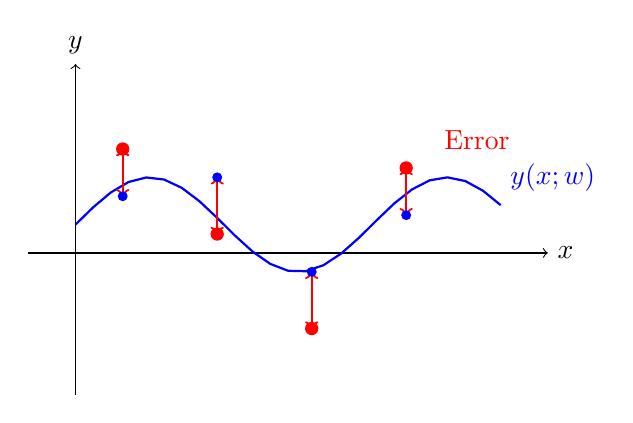
\begin{tikzpicture}[scale=1.2]
    \draw[->] (-0.5,0) -- (5,0) node[right] {$x$};
    \draw[->] (0,-1.5) -- (0,2) node[above] {$y$};
    
    % Fitted curve
    \draw[thick, blue, domain=0:4.5] plot (\x, {0.5*sin(2*\x r) + 0.3});
    
    % Data points and error bars
    \foreach \x/\y/\t in {0.5/0.6/1.1, 1.5/0.8/0.2, 2.5/-0.2/-0.8, 3.5/0.4/0.9} {
        \fill[red] (\x, \t) circle (2pt);
        \draw[red, thick, <->] (\x, \y) -- (\x, \t);
        \fill[blue] (\x, \y) circle (1.5pt);
    }
    
    % Labels
    \node[blue, right] at (4.5, 0.8) {$y(x; \vect{w})$};
    \node[red, right] at (3.8, 1.2) {Error};
\end{tikzpicture}
\end{center}

Each red line represents the error $(y(x_n; \vect{w}) - t_n)$. The squared error sums the squares of all these vertical distances.

\subsection{Mean Squared Error (MSE) and RMSE}

\begin{definitionbox}[Mean Squared Error and Root Mean Squared Error]
\textbf{Mean Squared Error (MSE)}:
\[
\text{MSE} = \frac{1}{N} \sum_{n=1}^{N} \left( y(x_n; \vect{w}) - t_n \right)^2
\]

\textbf{Root Mean Squared Error (RMSE)}:
\[
E_{\text{RMS}} = \sqrt{\frac{1}{N} \sum_{n=1}^{N} \left( y(x_n; \vect{w}) - t_n \right)^2}
\]
\end{definitionbox}

The RMSE has the same units as the target variable, making it more interpretable.

% ============================================================================
% OPTIMIZATION
% ============================================================================

\section{Finding the Optimal Parameters}

\subsection{The Optimization Problem}

We want to find the parameters $\vect{w}^*$ that minimize the error function:
\[
\vect{w}^* = \argmin_{\vect{w}} E(\vect{w})
\]

\subsection{Closed-Form Solution for Polynomial Fitting}

For polynomial regression with squared error, the solution can be found analytically. The normal equations yield:

\[
\vect{w}^* = (\mat{X}^\top \mat{X})^{-1} \mat{X}^\top \vect{t}
\]

where $\mat{X}$ is the \textbf{design matrix} with rows containing $(1, x_n, x_n^2, \ldots, x_n^M)$.

\begin{bluebox}[NumPy Implementation]
In practice, we use optimized implementations:
\begin{lstlisting}[language=Python]
import numpy as np

# Fit polynomial and get coefficients
coefficients = np.polyfit(x, t, degree)

# Create polynomial function
polynomial = np.poly1d(coefficients)

# Make predictions
predictions = polynomial(x_new)
\end{lstlisting}
\end{bluebox}

% ============================================================================
% OVERFITTING AND UNDERFITTING
% ============================================================================

\section{Overfitting and Underfitting}

\subsection{The Bias-Variance Tradeoff}

When we change the polynomial degree $M$, we observe a fundamental tension:

\begin{itemize}
    \item \textbf{Low $M$ (Underfitting)}: Model is too simple to capture the true pattern
    \item \textbf{High $M$ (Overfitting)}: Model is too complex and fits noise along with the pattern
\end{itemize}

\subsection{Visual Comparison}

\begin{center}
\renewcommand{\arraystretch}{1.5}
\begin{tabular}{|c|c|c|}
\hline
\textbf{Degree} & \textbf{Behavior} & \textbf{Result} \\ \hline
$M = 0$ & Constant line & Severe underfitting \\ \hline
$M = 1$ & Straight line & Underfitting \\ \hline
$M = 3$ & Cubic curve & \colorbox{green!20}{Good fit} \\ \hline
$M = 9$ & Passes through all points & Severe overfitting \\ \hline
\end{tabular}
\end{center}

\subsection{The Overfitting Paradox}

At $M = 9$ with $N = 10$ data points, the polynomial has 10 coefficients---exactly one per data point! This allows the curve to pass \textit{exactly} through every training point, achieving $E(\vect{w}) \approx 0$.

\begin{importantbox}[Zero Training Error Does Not Mean Good Model!]
A model with zero training error may have:
\begin{itemize}
    \item Memorized the training data (including noise)
    \item Learned nothing about the true underlying pattern
    \item Very poor predictions on new data (high test error)
\end{itemize}
\end{importantbox}

\subsection{Coefficient Explosion: The Root Cause}

When overfitting occurs, the coefficients $w_j$ take \textbf{extreme values}:

\begin{center}
\begin{tabular}{|c|c|c|c|c|}
\hline
\textbf{Degree} & $w_0$ & $w_1$ & $w_2$ & $\ldots$ \\ \hline
$M = 0$ & 0.12 & --- & --- & \\ \hline
$M = 1$ & 0.82 & -1.27 & --- & \\ \hline
$M = 3$ & 0.31 & 7.99 & -25.43 & 17.37 \\ \hline
$M = 9$ & 0.35 & 232.37 & -5321.83 & $\ldots$ (extreme) \\ \hline
\end{tabular}
\end{center}

Large coefficients mean the curve oscillates wildly to pass through each point.

\begin{bluebox}[Why Doesn't Higher Degree ``Include'' Lower?]
A natural question: Since a degree-9 polynomial can represent any degree-3 polynomial (by setting $w_4 = \cdots = w_9 = 0$), why doesn't it perform at least as well?

The answer: \textbf{The optimization finds the wrong solution.} With more parameters, there are many ways to achieve low training error, but most of them overfit. The optimization doesn't ``know'' to keep coefficients small.
\end{bluebox}

% ============================================================================
% REGULARIZATION
% ============================================================================

\section{Regularization: Controlling Complexity}

\subsection{The Key Insight}

We identified the problem: \textbf{coefficients become too large}. The solution: \textbf{penalize large coefficients} directly in the error function.

\subsection{Regularized Error Function}

\begin{definitionbox}[L2 Regularization (Ridge Regression)]
\[
\tilde{E}(\vect{w}) = \frac{1}{2} \sum_{n=1}^{N} \left( y(x_n; \vect{w}) - t_n \right)^2 + \frac{\lambda}{2} \|\vect{w}\|^2
\]
where:
\begin{itemize}
    \item $\|\vect{w}\|^2 = \sum_{j=0}^{M} w_j^2 = \vect{w}^\top \vect{w}$ is the squared L2 norm
    \item $\lambda \geq 0$ is the \textbf{regularization parameter}
\end{itemize}
\end{definitionbox}

\subsection{The Tug-of-War}

The regularized objective creates a balance:

\begin{center}
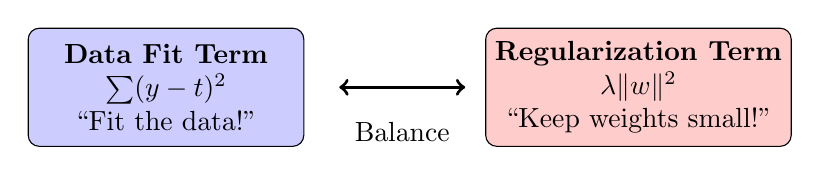
\begin{tikzpicture}[
    box/.style={draw, rounded corners, minimum width=3.5cm, minimum height=1.5cm, align=center}
]
    \node[box, fill=blue!20] (fit) at (-3,0) {\textbf{Data Fit Term}\\$\sum (y - t)^2$\\``Fit the data!''};
    \node[box, fill=red!20] (reg) at (3,0) {\textbf{Regularization Term}\\$\lambda \|\vect{w}\|^2$\\``Keep weights small!''};
    
    \draw[very thick, <->] (-0.8,0) -- (0.8,0) node[midway, below=0.3cm] {Balance};
\end{tikzpicture}
\end{center}

\begin{itemize}
    \item If $\lambda = 0$: No regularization, potential overfitting
    \item If $\lambda$ is very large: Weights forced toward zero, potential underfitting
    \item Optimal $\lambda$: Balances fit quality with model simplicity
\end{itemize}

\subsection{Effect of Regularization}

With proper regularization, even a degree-9 polynomial can avoid overfitting:

\begin{itemize}
    \item \textbf{Without regularization ($\lambda = 0$)}: Wild oscillations, passing through all points
    \item \textbf{With regularization ($\lambda$ optimal)}: Smooth curve approximating $\sin(2\pi x)$
\end{itemize}

\begin{bluebox}[Alternative Names]
\begin{itemize}
    \item \textbf{Ridge Regression}: Statistical term for L2 regularization
    \item \textbf{Weight Decay}: Neural network term (weights ``decay'' toward zero)
    \item \textbf{Shrinkage}: Coefficients are ``shrunk'' toward zero
    \item \textbf{Tikhonov Regularization}: Mathematical term
\end{itemize}
\end{bluebox}

% ============================================================================
% HYPERPARAMETERS AND VALIDATION
% ============================================================================

\section{Hyperparameters and Validation}

\subsection{Parameters vs. Hyperparameters}

\begin{definitionbox}[Parameters and Hyperparameters]
\textbf{Parameters} ($\vect{w}$):
\begin{itemize}
    \item Learned from data during training
    \item Found by minimizing the error function
\end{itemize}

\textbf{Hyperparameters} ($M$, $\lambda$):
\begin{itemize}
    \item Set \textit{before} training
    \item Not learned from data (or learned separately)
    \item Control model structure and regularization
\end{itemize}
\end{definitionbox}

\subsection{Why Not Optimize Hyperparameters Jointly?}

A natural question: Why not minimize $\tilde{E}(\vect{w}, \lambda)$ jointly over $\vect{w}$ and $\lambda$?

\textbf{Answer}: The optimization would set $\lambda = 0$ and overfit! The regularization term fights against the objective, so joint optimization eliminates it.

\subsection{Train, Validation, and Test Sets}

To properly tune hyperparameters and evaluate the model:

\begin{center}
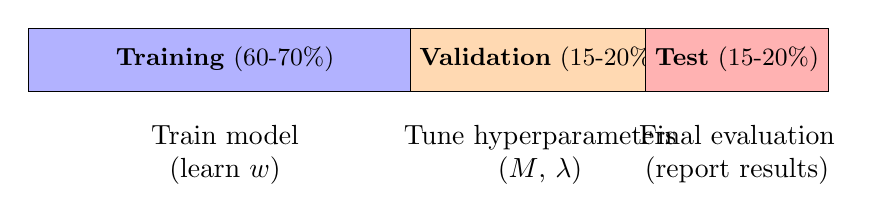
\begin{tikzpicture}[
    set/.style={draw, minimum height=0.8cm, align=center, font=\small}
]
    \node[set, fill=blue!30, minimum width=5cm] (train) at (0,0) {\textbf{Training} (60-70\%)};
    \node[set, fill=orange!30, minimum width=2cm] (val) at (4,0) {\textbf{Validation} (15-20\%)};
    \node[set, fill=red!30, minimum width=2cm] (test) at (6.5,0) {\textbf{Test} (15-20\%)};
    
    \node[below=0.3cm, align=center] at (train.south) {Train model\\(learn $\vect{w}$)};
    \node[below=0.3cm, align=center] at (val.south) {Tune hyperparameters\\($M$, $\lambda$)};
    \node[below=0.3cm, align=center] at (test.south) {Final evaluation\\(report results)};
\end{tikzpicture}
\end{center}

\subsection{The Validation Process}

\begin{enumerate}
    \item \textbf{Choose} candidate hyperparameter values (e.g., $\lambda \in \{0.001, 0.01, 0.1, 1\}$)
    \item \textbf{For each} candidate:
    \begin{enumerate}
        \item Train model on training set (find optimal $\vect{w}$)
        \item Evaluate on validation set (compute validation error)
    \end{enumerate}
    \item \textbf{Select} hyperparameters with lowest validation error
    \item \textbf{Retrain} on training + validation data with best hyperparameters
    \item \textbf{Report} final performance on test set
\end{enumerate}

\begin{importantbox}[Never Train on Test Data!]
The test set must remain completely unseen during model development. If you tune hyperparameters based on test performance, you're effectively training on the test set, and your reported performance will be overly optimistic.
\end{importantbox}

\subsection{Cross-Validation}

When data is limited, we use \textbf{k-fold cross-validation}:

\begin{enumerate}
    \item Divide data into $k$ equal folds
    \item For $i = 1, \ldots, k$:
    \begin{itemize}
        \item Use fold $i$ as validation, rest as training
        \item Record validation error
    \end{itemize}
    \item Average the $k$ validation errors
\end{enumerate}

Common choices: $k = 5$ or $k = 10$.

% ============================================================================
% SUMMARY
% ============================================================================

\section{Chapter Summary}

\begin{itemize}
    \item \textbf{Data generation}: Real-world data combines a pattern (signal) and noise. Our goal is to learn the pattern.
    
    \item \textbf{Curve fitting}: We fit a parameterized function (e.g., polynomial) to data by adjusting parameters $\vect{w}$.
    
    \item \textbf{Error function}: Quantifies fit quality. Sum of squared errors is common:
    \[
    E(\vect{w}) = \frac{1}{2} \sum_{n=1}^{N} (y(x_n; \vect{w}) - t_n)^2
    \]
    
    \item \textbf{Overfitting}: Occurs when the model is too complex. Signs include:
    \begin{itemize}
        \item Very low training error but high test error
        \item Extreme coefficient values
        \item Curve oscillating wildly to pass through all points
    \end{itemize}
    
    \item \textbf{Regularization}: Penalizes large coefficients to prevent overfitting:
    \[
    \tilde{E}(\vect{w}) = E(\vect{w}) + \frac{\lambda}{2} \|\vect{w}\|^2
    \]
    
    \item \textbf{Hyperparameters}: $M$ (polynomial degree) and $\lambda$ (regularization strength) are set before training and tuned via validation.
    
    \item \textbf{Generalization}: The ultimate goal is good performance on unseen data, not just fitting training data.
\end{itemize}

\begin{bluebox}[Key Takeaways for Practice]
\begin{enumerate}
    \item More parameters $\neq$ better model (if unconstrained)
    \item Always use a held-out test set for final evaluation
    \item Regularization is essential when model capacity exceeds data size
    \item Low training error is not sufficient; track validation error too
    \item Hyperparameter tuning is as important as model selection
\end{enumerate}
\end{bluebox}
